\section{Annexe : tableau de transformées de Fourier}

This table of transformées de Fourier is the one document allowed in the exam, which
is otherwise sat without documents and without a calculator; the table is
supplied. The table below keeps its notation, symbols and sign convention.

\subsection{Variables duales}

\begin{notation}[Espaces duaux]
  The table is written once, in a neutral pair of variables: $\xi$ et $\Xi$
  sont les variables de deux espaces duaux (lettre grecque ksi/xi minuscule et
  majuscule). The transformée de Fourier inverse (left column) and the
  transformée directe (right column) are
  \[
    f(\xi)=\int_{-\infty}^{+\infty}F(\Xi)\exp(2j\pi\xi\Xi)\,d\Xi,
    \qquad
    F(\Xi)=\int_{-\infty}^{+\infty}f(\xi)\exp(-2j\pi\xi\Xi)\,d\xi .
  \]
  The kernel carries $2\pi$ in the exponent, not $\omega$, so there is no
  $1/2\pi$ prefactor anywhere in the table. The engineering $j$ is used, not $i$.
\end{notation}

The table then gives the two substitutions the course actually needs.

\begin{notation}[The two readings of the table]
  \textbf{Temps / fréquences}~:
  \[
    f(t)=\int_{-\infty}^{+\infty}F(\nu)\exp(j2\pi\nu t)\,d\nu
    \qquad\lra\qquad \xi=t \ \text{ and }\ \Xi=\nu .
  \]
  \textbf{Espace / Fréquences spatiales}~:
  \[
    F(x)=\int_{-\infty}^{+\infty}f(u)\exp(-j2\pi ux)\,du
    \qquad\lra\qquad \xi=u \ \text{ and }\ \Xi=x .
  \]
\end{notation}

\begin{remark}
  The two substitutions are not parallel, and this is the commonest way to read
  the table backwards. In the temporal reading the lower-case variable is the
  \emph{signal} variable $t$ and the upper-case one the \emph{frequency} $\nu$.
  In the spatial reading it is the other way round: the lower-case $\xi$ is the
  \emph{fréquence spatiale} $u$ and the upper-case $\Xi$ is the \emph{space}
  variable $x$. So in diffraction the minus-sign integral --- the right-hand
  column --- is the one that carries you from the plane of fréquences spatiales
  back to the object plane, and a pair read left-to-right off the table is a
  $u\to x$ pair, not an $x\to u$ one.
\end{remark}

\subsection{Fonctions d'une seule variable}

\begin{table}[h!]
  \centering
  \begin{tabularx}{\textwidth}{>{\centering\arraybackslash}X >{\centering\arraybackslash}X}
    \toprule
    $\xi$ & $\Xi$ \\
    \midrule
    $\delta(\xi)$ = « delta de Dirac » & $1$ \\[6pt]
    $\delta(\xi-\xi_0)$ & $\exp(-2j\pi\xi_0\Xi)$ \\[6pt]
    $1$ & $\delta(\Xi)$ \\[6pt]
    $\exp(+2j\pi\xi\Xi_0)$ & $\delta(\Xi-\Xi_0)$ \\[6pt]
    $\sin(2\pi\xi\Xi_0)$ &
      $\dfrac{j}{2}\left[\delta(\Xi+\Xi_0)-\delta(\Xi-\Xi_0)\right]$ \\[10pt]
    $\cos(2\pi\xi\Xi_0)$ &
      $\dfrac{1}{2}\left[\delta(\Xi+\Xi_0)+\delta(\Xi-\Xi_0)\right]$ \\
    \bottomrule
  \end{tabularx}
\end{table}

\begin{table}[h!]
  \centering
  \begin{tabularx}{\textwidth}{>{\centering\arraybackslash}X >{\centering\arraybackslash}X}
    \toprule
    $\xi$ & $\Xi$ \\
    \midrule
    $\operatorname{Sign}(\xi)=
      \begin{cases}
        \phantom{-}1 & \text{pour } \xi>0\\
        \phantom{-}0 & \text{pour } \xi=0\\
        -1 & \text{pour } \xi<0
      \end{cases}$
    & $\dfrac{1}{j\pi\Xi}$ \\[16pt]
    $-\dfrac{1}{j\pi\xi}$
    & $\operatorname{Sign}(\Xi)=
      \begin{cases}
        \phantom{-}1 & \text{pour } \Xi>0\\
        \phantom{-}0 & \text{pour } \Xi=0\\
        -1 & \text{pour } \Xi<0
      \end{cases}$ \\[16pt]
    $\operatorname{Step}(\xi)=
      \begin{cases}
        1 & \text{pour } \xi>0\\
        0{,}5 & \text{pour } \xi=0\\
        0 & \text{pour } \xi<0
      \end{cases}$
    & $\dfrac{1}{2}\left[\delta(\Xi)+\dfrac{1}{j\pi\Xi}\right]$ \\[16pt]
    $\dfrac{1}{2}\left[\delta(\xi)-\dfrac{1}{j\pi\xi}\right]$
    & $\operatorname{Step}(\Xi)=
      \begin{cases}
        1 & \text{pour } \Xi>0\\
        0{,}5 & \text{pour } \Xi=0\\
        0 & \text{pour } \Xi<0
      \end{cases}$ \\
    \bottomrule
  \end{tabularx}
\end{table}

\begin{table}[h!]
  \centering
  \begin{tabularx}{\textwidth}{>{\centering\arraybackslash}X >{\centering\arraybackslash}X}
    \toprule
    $\xi$ & $\Xi$ \\
    \midrule
    $\boldsymbol{\omega}_L(\xi)=\displaystyle\sum_{n=-\infty}^{+\infty}\delta(\xi-nL)
      =\frac{1}{L}\sum_{n=-\infty}^{+\infty}\exp\!\left(j\frac{2\pi n\xi}{L}\right)$
    & $\dfrac{1}{L}\,\boldsymbol{\omega}_{1/L}(\Xi)
      =\dfrac{1}{L}\displaystyle\sum_{n=-\infty}^{+\infty}\delta\!\left(\Xi-\frac{n}{L}\right)
      =\sum_{n=-\infty}^{+\infty}\exp(j2\pi nL\Xi)$ \\[22pt]
    $\boldsymbol{\pi}_L(\xi)=\boldsymbol{\pi}\!\left(\dfrac{\xi}{L}\right)=
      \begin{cases}
        1 & \text{si } |\xi|<\dfrac{L}{2}\\[4pt]
        0 & \text{sinon}
      \end{cases}$
    & $L\,\dfrac{\sin \pi\Xi L}{\pi\Xi L}=L\operatorname{Sinc}(\pi\Xi L)$ \\[16pt]
    $L\,\dfrac{\sin \pi\xi L}{\pi\xi L}=L\sinc(\pi\xi L)$
    & $\boldsymbol{\pi}_L(\Xi)=\boldsymbol{\pi}\!\left(\dfrac{\Xi}{L}\right)=
      \begin{cases}
        1 & \text{si } |\Xi|<\dfrac{L}{2}\\[4pt]
        0 & \text{sinon}
      \end{cases}$ \\[16pt]
    $\operatorname{Sinc}^2(\xi)$ & $\operatorname{tri}(\Xi)$ \\[6pt]
    $\operatorname{tri}(\xi)$ & $\operatorname{Sinc}^2(\Xi)$ \\[6pt]
    $\operatorname{Gauss}\!\left(\dfrac{\xi}{L}\right)=\exp\!\left(-\pi\dfrac{\xi^2}{L^2}\right)$
    & $L\operatorname{Gauss}(L\Xi)=L\exp(-\pi L^2\Xi^2)$ \\[12pt]
    $\cos(\pi\xi^2)$ & $\cos\!\left(\pi\left(\Xi^2-\dfrac{1}{4}\right)\right)$ \\[12pt]
    $\sin(\pi\xi^2)$ & $-\sin\!\left(\pi\left(\Xi^2-\dfrac{1}{4}\right)\right)$ \\
    \bottomrule
  \end{tabularx}
\end{table}

\clearpage

\begin{remark}[Reading the table's own function names]
  $\boldsymbol{\pi}$ is the porte of unit height, so
  $\boldsymbol{\pi}_L$ has \emph{total width} $L$ and the condition is
  $|\xi|<L/2$. $\boldsymbol{\omega}_L$ is the peigne de Dirac of period $L$,
  poids $1$. $\operatorname{tri}$ is
  the unit triangle. $\operatorname{Gauss}$ is normalised so that
  $\operatorname{Gauss}(0)=1$ and the $\pi$ sits in the exponent, which is
  exactly what makes the Gaussian its own transform up to the $L$ scaling.
\end{remark}

\begin{remark}[The table uses two different $\sinc$ conventions]
  In the porte rows the table spells the meaning out,
  $L\,\frac{\sin\pi\xi L}{\pi\xi L}=L\sinc(\pi\xi L)$, so there
  $\sinc(x)=\sin x/x$ and the $\pi$ is already written into the argument;
  feeding such a row an argument without the $\pi$ is the fastest way to lose a
  factor of $\pi$ in a diffraction calculation. The
  $\operatorname{Sinc}^2\lra\operatorname{tri}$ rows, by contrast, are printed
  with no $\pi$ anywhere in the argument and are correct only for the
  \emph{normalised} $\operatorname{Sinc}(x)=\sin(\pi x)/(\pi x)$: read them the
  unnormalised way and $\left(\frac{\sin\xi}{\xi}\right)^2$ transforms to
  $\pi\operatorname{tri}(\pi\Xi)$, not $\operatorname{tri}(\Xi)$. The table
  gives both conventions the same name (spelt $L\,sinc$ in one row and
  $L\,Sinc$ or $\operatorname{Sinc}^2$ elsewhere; the capitalisation carries no
  meaning), so read each row by whether the $\pi$ is written.
\end{remark}

\begin{remark}[Le poids du peigne]
  The transform of a peigne de Dirac of period $L$ and unit poids is a peigne of
  period $1/L$ carrying poids $1/L$, not $1$. The second equality in each cell
  is the Poisson summation identity; it is the entry the sampling arguments of the
  diffraction chapter rest on, and the $1/L$ is the part most often dropped.
\end{remark}

\begin{figure}[h!]
  \centering
  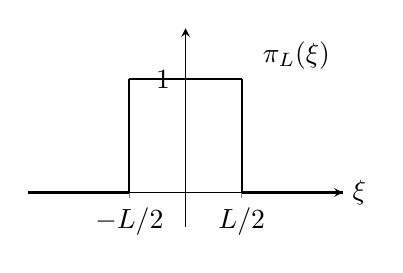
\begin{tikzpicture}
    \begin{axis}[
      width=0.46\textwidth, height=4.1cm,
      axis lines=middle, xlabel={$\xi$},
      xtick={-1,1}, xticklabels={$-L/2$,$L/2$},
      ytick={1}, yticklabels={$1$},
      xmin=-2.8, xmax=2.8, ymin=-0.3, ymax=1.45,
      every axis x label/.style={at={(ticklabel* cs:1.0)},anchor=west},
      ]
      \addplot[thick,domain=-2.8:-1,samples=2]{0};
      \addplot[thick,domain=-1:1,samples=2]{1};
      \addplot[thick,domain=1:2.8,samples=2]{0};
      \draw[thick] (axis cs:-1,0) -- (axis cs:-1,1);
      \draw[thick] (axis cs:1,1) -- (axis cs:1,0);
      \node[anchor=south west] at (axis cs:1.2,1.0) {$\boldsymbol{\pi}_L(\xi)$};
    \end{axis}
  \end{tikzpicture}
  \hfill
  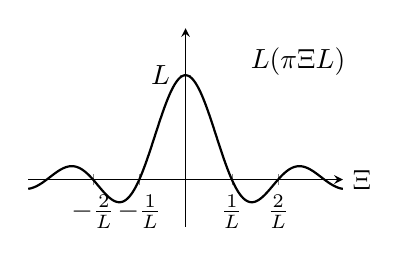
\begin{tikzpicture}
    \begin{axis}[
      width=0.46\textwidth, height=4.1cm,
      axis lines=middle, xlabel={$\Xi$},
      xtick={-2,-1,1,2}, xticklabels={$-\frac{2}{L}$,$-\frac{1}{L}$,$\frac{1}{L}$,$\frac{2}{L}$},
      ytick={1}, yticklabels={$L$},
      xmin=-3.4, xmax=3.4, ymin=-0.45, ymax=1.45,
      every axis x label/.style={at={(ticklabel* cs:1.0)},anchor=west},
      ]
      \addplot[thick,domain=-3.4:3.4,samples=200]{sin(deg(pi*x))/(pi*x)};
      \node[anchor=south west] at (axis cs:1.2,0.9) {$L\sinc(\pi\Xi L)$};
    \end{axis}
  \end{tikzpicture}
  \caption*{}
\end{figure}

\begin{figure}[h!]
  \centering
  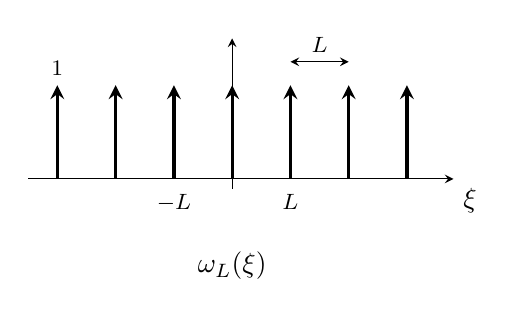
\begin{tikzpicture}[>=stealth, xscale=0.74, yscale=0.85]
    \draw[->] (-3.5,0) -- (3.8,0) node[below right] {$\xi$};
    \draw[->] (0,-0.15) -- (0,2.1);
    \foreach \x in {-3,-2,-1,0,1,2,3} \draw[->,very thick] (\x,0) -- (\x,1.4);
    \draw[<->] (1,1.75) -- (2,1.75) node[midway,above] {\footnotesize $L$};
    \node[anchor=south] at (-3,1.4) {\footnotesize $1$};
    \node[anchor=north] at (1,-0.08) {\footnotesize $L$};
    \node[anchor=north] at (-1,-0.08) {\footnotesize $-L$};
    \node at (0,-1.3) {$\boldsymbol{\omega}_L(\xi)$};
  \end{tikzpicture}
  \hspace{0.015\textwidth}
  \begin{tikzpicture}[>=stealth, xscale=0.74, yscale=0.85]
    \draw[->] (-3.5,0) -- (3.8,0) node[below right] {$\Xi$};
    \draw[->] (0,-0.15) -- (0,2.1);
    \foreach \x in {-3,-2.5,-2,-1.5,-1,-0.5,0,0.5,1,1.5,2,2.5,3}
      \draw[->,very thick] (\x,0) -- (\x,0.7);
    \draw[<->] (2,1.75) -- (2.5,1.75) node[midway,above] {\footnotesize $1/L$};
    \node[anchor=south] at (-3,0.7) {\footnotesize $\tfrac{1}{L}$};
    \node[anchor=north] at (1,-0.08) {\footnotesize $\tfrac{2}{L}$};
    \node[anchor=north] at (-1,-0.08) {\footnotesize $-\tfrac{2}{L}$};
    \node at (0,-1.3) {$\tfrac{1}{L}\boldsymbol{\omega}_{1/L}(\Xi)$};
  \end{tikzpicture}
  \caption*{}
\end{figure}

\subsection{Fonctions de deux variables}

Ce tableau s'applique pour le cas de la diffraction, c'est-à-dire de l'espace
$(x,y)$ à l'espace des fréquences spatiales $(u,v)$.

\begin{table}[h!]
  \centering
  \begin{tabularx}{\textwidth}{>{\centering\arraybackslash}X >{\centering\arraybackslash}X}
    \toprule
    $\displaystyle f(\v{\rho})=\int_{-\infty}^{+\infty}F(\v{r})\exp(2j\pi \v{r}\v{\rho})\,d^2\v{r}$
      \newline \textit{Avec} $\v{\rho}(u,v)$
    & $\displaystyle F(\v{r})=\int_{-\infty}^{+\infty}f(\v{\rho})\exp(-2j\pi \v{r}\v{\rho})\,d^2\v{\rho}$
      \newline \textit{Avec} $\v{r}(x,y)$ \\
    \midrule
    $f(u)\,g(v)$
    & $F(x)\,G(y)$ \newline \textit{fonction à variables séparables} \\[8pt]
    $1(u)\,1(v)$ & $\delta(x,y)$ \\[8pt]
    $\dfrac{\pi D^2}{4}\operatorname{Somb}(\rho D)
      =\dfrac{\pi D^2}{4}\,\dfrac{2J_1(\pi\rho D)}{\pi\rho D}$
    & $\operatorname{Circ}\!\left(\dfrac{r}{D}\right)=
      \begin{cases}
        1 & \text{pour } r\le \dfrac{D}{2}\\[6pt]
        0 & \text{pour } r\ge \dfrac{D}{2}
      \end{cases}$ \\[20pt]
    $r_0^2\operatorname{Gauss}(\rho r_0)=r_0^2\exp(-\pi r_0^2\rho^2)$
    & $\operatorname{Gauss}\!\left(\dfrac{r}{r_0}\right)
      =\exp\!\left(-\pi\dfrac{r^2}{r_0^2}\right)$ \\
    \bottomrule
  \end{tabularx}
\end{table}

\begin{remark}[The second table's variables and its Bessel function]
  The right-hand column's variable is $\v{r}(x,y)$: the whole point of the
  second table is that $\v{\rho}$ lives in the plane of fréquences spatiales
  $(u,v)$ and $\v{r}$ in the object plane $(x,y)$, as the rows
  $f(u)g(v)\lra F(x)G(y)$ and $\operatorname{Circ}(r/D)$ make plain.\\

  The $\operatorname{Somb}$ entry carries $J_1$, the fonction de Bessel de
  première espèce of order one, and not $J_0$. With $J_0$ the expression would
  diverge at $\rho=0$, since $J_0(0)=1$ and the $\pi\rho D$ in the denominator
  vanishes, whereas the value at the origin must be the aperture area
  $\pi D^2/4$. Only $2J_1(x)/x\to 1$ as $x\to 0$ does that, and it is $J_1$
  whose first zero at $x=1{,}22\pi$ gives the Airy radius.
\end{remark}

\begin{remark}
  $\operatorname{Circ}(r/D)$ is written in terms of the \emph{diameter} $D$, not
  the radius, so its support is $r\le D/2$ and its area is $\pi D^2/4$ --- which
  is the prefactor in front of $\operatorname{Somb}$, as it must be. Likewise
  $\operatorname{Gauss}(r/r_0)$ uses the $1/e$-of-$\pi$ radius $r_0$, and the
  transform picks up $r_0^2$, one power of $r_0$ per dimension, against the
  single power of $L$ in the one-variable table.
\end{remark}

\subsection{Autres paires à deux dimensions}

Four further two-dimensional pairs complete the table. They do not follow the
notation of the tables above: the peigne is written $\mathrm{III}$ rather than
$\boldsymbol{\omega}$, the imaginary unit is $i$ rather than $j$, and the
two-dimensional Dirac is $\delta^2(x,y)$ rather than $\delta(x,y)$.

\begin{table}[h!]
  \centering
  \begin{tabularx}{\textwidth}{>{\centering\arraybackslash}X >{\centering\arraybackslash}X}
    \toprule
    $(x,y)$ & $(u,v)$ \\
    \midrule
    $\delta^2(x,y)$ & $1$ \\[6pt]
    $\mathrm{III}(y)\,\delta(x)$ & $\mathrm{III}(v)$ \\[6pt]
    $\exp\!\left(-\pi\dfrac{x^2+y^2}{a^2}\right)$ & $a^2\exp\!\left(-\pi a^2(u^2+v^2)\right)$ \\[12pt]
    $\sin \pi y$
    & $\dfrac{i}{2}\,\delta^2\!\left(u,v-\dfrac{1}{2}\right)
      -\dfrac{i}{2}\,\delta^2\!\left(u,v+\dfrac{1}{2}\right)$ \\
    \bottomrule
  \end{tabularx}
\end{table}

\begin{remark}[These pairs use the opposite sign convention]
  The last row contradicts the one-variable table. With the table's kernel
  $\exp(-2j\pi\xi\Xi)$, the entry $\sin(2\pi\xi\Xi_0)\lra
  \frac{j}{2}\left[\delta(\Xi+\Xi_0)-\delta(\Xi-\Xi_0)\right]$ applied to
  $\sin\pi y=\sin(2\pi\cdot\tfrac12\cdot y)$ gives
  $\frac{j}{2}\left[\delta(v+\tfrac12)-\delta(v-\tfrac12)\right]$ --- the
  opposite sign to the last row, which is written with the conjugate kernel
  $\exp(+2i\pi)$. Use the one-variable table's sign, since that is the one the
  rest of the course and the exam follow.\\

  The Gaussian row's transform is $a^2\exp(-\pi a^2(u^2+v^2))$, with one power
  of $a$ per dimension, like the $r_0^2$ of the two-variable table above.
\end{remark}

\subsection{Ce que le tableau ne donne pas}

\begin{remark}
  The table is a table of \emph{pairs} only. It carries no properties or
  theorems section: linéarité, changement d'échelle, translation ou déphasage
  and the théorème de Parseval-Plancherel belong to chapter 2 and are \emph{not} handed out. Neither is the théorème de
  convolution. Those have to be carried into the room in your head; only the
  pairs above are on the desk.
\end{remark}

A short bibliography for the course: L. Léger, \textit{Cours d'optique
géométrique et ondulatoire} (Orsay, 1992); B. Saleh and
M. Teich, \textit{Fundamentals of Photonics} (Wiley, 1991); I. and M. Joindot,
\textit{Les télécommunications par fibres optiques} (Dunod, 1996); J.-P. Pérez,
\textit{Optique géométrique et ondulatoire} (Masson, 1994); G. M. Stéphan,
\textit{Cours d'optique de Fourier} (Rennes, 1996).
